\documentclass[
    a4paper,
    12pt,
    oneside
]{report}

% Import packages
\usepackage{graphicx}
\usepackage{subfigure}
\usepackage{amsmath}  % Replaced latexsym with amsmath for symbols and mathematical operations
\usepackage[utf8]{inputenc}
\usepackage[english]{babel}
\usepackage{pdfpages}
\usepackage[
    backend=biber,
    style=ieee
]{biblatex} % IEEE style citations
\usepackage{csquotes}
\usepackage{url}
\usepackage[T1]{fontenc}
\usepackage{float}
\usepackage{palatino}
\usepackage{color}
\usepackage{algorithm}
\usepackage{algorithmic}

\setlength{\doublerulesep}{\arrayrulewidth}
% \setlength{\textwidth}{16cm}
% \setlength{\textheight}{24cm}
% \setlength{\hoffset}{-1.7cm} 
% \setlength{\voffset}{-1cm}
% \setlength{\topmargin}{-0.5cm} 
% \setlength{\footskip}{27pt}
\usepackage[a4paper, margin=2.5cm]{geometry}

\renewcommand{\baselinestretch}{1.3}
\linespread{1}

\usepackage{titlesec}
\titlespacing*{\chapter}{0pt}{-1\baselineskip}{1\baselineskip}
\titlespacing*{\section}{0pt}{\baselineskip}{0pt}

\usepackage{fancyhdr}

\fancypagestyle{noheadrule}{
    \fancyhf{}
    \renewcommand{\headrulewidth}{0pt}
    \renewcommand{\footrulewidth}{0.5pt}
    \fancyfoot[L,LO]{\textit {FINAL PROJECT: Collective Transport using
    Decentralised Swarm Robotics}}
    \fancyfoot[R,RO]{\bfseries\thepage}
}

% Add bibliography file to document
\addbibresource{biblio.bib}

\begin{document}

% Cover
\begin{titlepage}
    \centering
    % \vspace*{1cm}

    {\LARGE \textbf{Final Project I}}\\[1cm]
    {\Huge \textbf{Collective Transport using Decentralised Swarm Robotics}}\\[1cm]

    
\includegraphics[width=0.4\textwidth]{assets/images/ise_logo.png}\\[1cm]
    
    \textbf{Submitted to the}\\[0.1cm]
    Project Committee appointed by the\\
    \textbf{International School of Engineering (ISE)}\\
    Faculty of Engineering, Chulalongkorn University\\[1cm]

    \textbf{Project Adviser}\\[0.1cm]
    Asst.Prof.Paulo Fernando Rocha Garcia, Ph.D.\\[1cm]

    \textbf{Submitted By}\\[0.5cm]
    \begin{tabular}{rl}
        6438067021 & Nattadon Tangsasom \\
        6438075021 & Ting-Yi Lin \\
        6438079621 & Tinapat Limsila \\
        6438118421 & Noppawan Srikhirin \\
        6438187721 & Mehul Sharma \\
    \end{tabular}\\[1cm]
    2/2024: 2147417 Final Project II\\
    Robotics and Artificial Intelligence Engineering (International Programme)\\
    International School of Engineering (ISE) Faculty of Engineering, Chulalongkorn University

\end{titlepage}


\thispagestyle{empty}
\pagenumbering{roman} \setcounter{page}{1}
\setcounter{secnumdepth}{11}
\setcounter{tocdepth}{3}
\renewcommand{\chaptermark}[1]{\markboth{Chapter ~\thechapter~:~#1}{}}
\fancyhf{}
\fancyhead[R,RO]{\bfseries\leftmark}
\fancyfoot[L,LO]{\textit {FINAL PROJECT: Collective Transport using
Decentralised Swarm Robotics}} 
\fancyfoot[R,RO]{\bfseries\thepage}
\fancypagestyle{plain}{
    \fancyhead{}
    \renewcommand{\headrulewidth}{0pt}
} 
\pagestyle{fancy}
\selectlanguage{english}
{\linespread{.8}\tableofcontents}
\newpage
\pagenumbering{arabic}
\titlespacing{\chapter}{0cm}{1cm}{2cm}

% Chapters
\chapter*{Abstract}

\paragraph*{}
This report serves as the proposal for our final project, titled "Collective Transport using Swarm Robotics." It covers various facets of our project, including the project concept, expected outcomes, project timeline, and potential benefits to the industry. Additionally, a comprehensive review of existing literature and a robust theoretical foundation are provided to substantiate our objectives.

\paragraph*{}
Structured into nine chapters, the report begins with an exploration of the research background and our objectives. The literature survey evaluates multiple research papers to identify relevant concepts, enhancing and applying them in innovative ways. Subsequent chapters delve into the development of the project concept, detailing the planning and execution strategy. A theoretical backup section fortifies our project methodology. The anticipated project outcomes are discussed, followed by the potential benefits to the industry. The report concludes by outlining each team member's contributions to the project.

\paragraph*{}
As a proposal for our final project, this report is intended to outline our plans and should not be considered as a finalized product. The comprehensive information provided across the nine chapters aims to furnish sufficient details for an effective project proposal.

\chapter{Introduction}

\paragraph*{}
This progress report aims to highlight the progress of our final project, \textbf{Collective Transport using Swarm Robotics}, with the evaluating criteria being the team individual contributions, as well as our pace in comparison to the ideal schedule. The ideal schedule can be represented by the project Gantt Chart (Figure \ref{fig:gantt_chart}).

\paragraph*{}
According to Figure \ref{fig:gantt_chart}, we are exploring three major sub-tasks during this iteration of the project schedule. These three tasks are: \textbf{Communication in the Swarm} (Task 1.1), \textbf{Object detection using Computer Vision} (Task 1.2), and \textbf{Simple Simultaneous Localization and Mapping} (Task 1.3). These tasks are planned to span for the entire month of September. Two team members, one team member, and two team members are assigned to each task, respectively.

\begin{figure}[H]
    \centering
    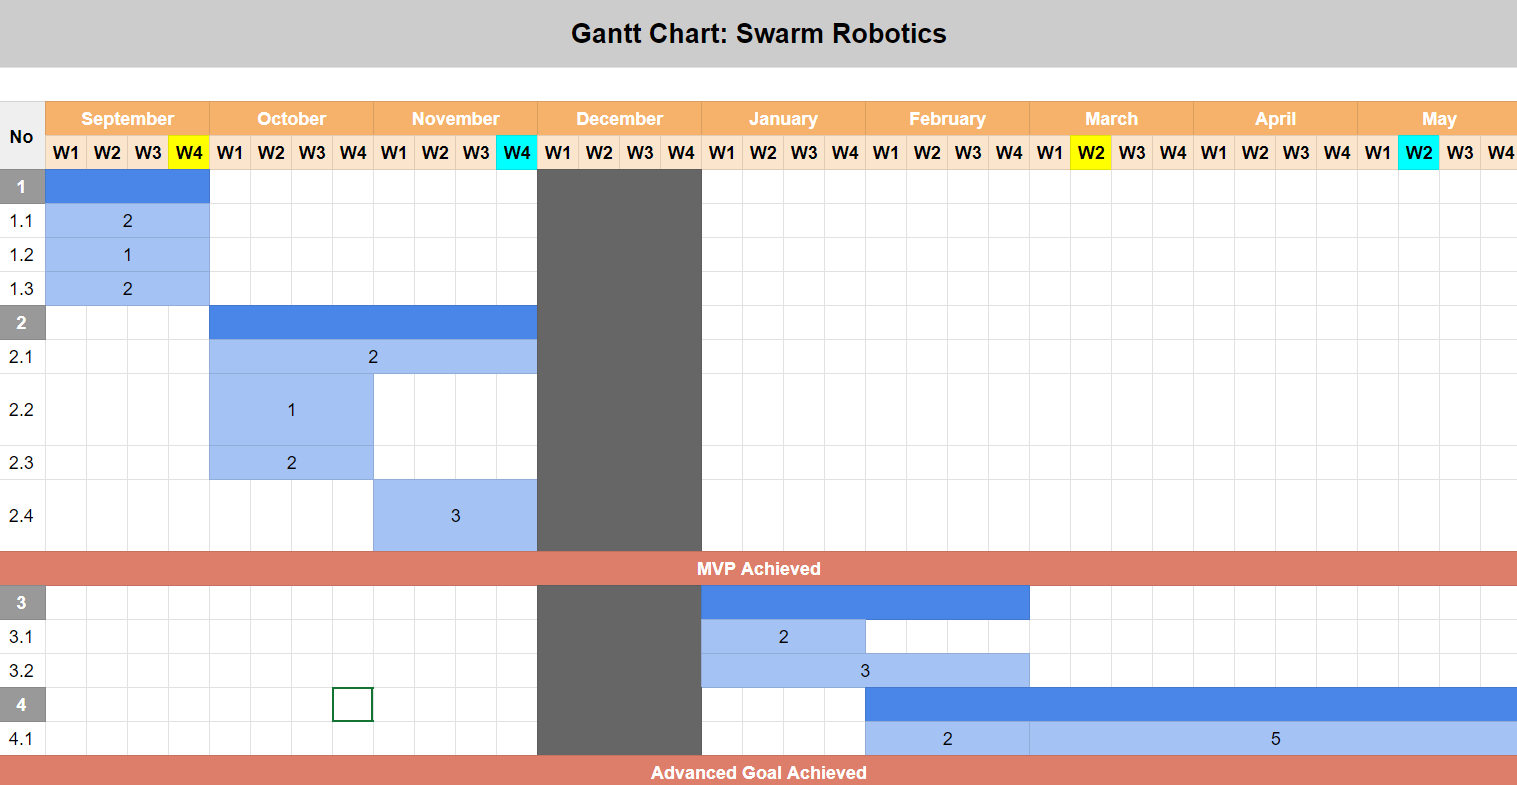
\includegraphics[width=1\linewidth]{progress_report_1/assets/images/introduction/gantt_chart.png}
    \caption{Project Gantt Chart}
    \label{fig:gantt_chart}
\end{figure}

\chapter{Conclusion}

\paragraph*{}
Swarm communication has been successfully implemented using a decentralized peer-to-peer architecture facilitated by socket communication. This approach was selected for its low latency and reliability, both of which are essential for real-time data exchange among robots. A three-way handshake mechanism was incorporated to ensure message delivery integrity, along with a consensus algorithm to resolve simultaneous object detection and taskmaster assignment conflicts. With coordinate streaming, dynamic path planning, and task execution now fully integrated, the communication system provides a solid foundation for coordinated swarm behavior, enabling seamless transitions between detection, planning, and movement phases.

\paragraph*{}
Additionally, the object detection system utilizing multi-sensor fusion of the camera and S3 RPLiDAR accurately measures relative distance, relative angle, and estimated width, aided by the variation factor function. This function yields an error margin of 1 centimeter for cylinders with diameters of 16 and 20 centimeters. The model was also tested with objects of different sizes, specifically a cylinder with a diameter of 12 centimeters, resulting in a slightly higher error margin of 2 centimeters. Overall, the object detection component was completed within the expected timeline.

\paragraph*{}
For SLAM we will continue making our own graph SLAM but will work on SLAM Toolbox temporarily. For odometry, we will continue testing and publish results soon.

\paragraph*{}
Meanwhile, the development and testing of our holonomic X-Drive robot have progressed significantly. The robot’s base and structural components were 3D printed using PLA, but to improve durability and stability, key parts such as the baseplate, shaft, wheels, and flange coupler will be upgraded to acrylic and stainless steel. The robot utilizes Dynamixel AX-12W motors for enhanced back-drivability, controlled through a custom ROS 2 package that applies a Jacobian matrix transformation for motion control. Transitioning from the older Maxon BLDC motors has streamlined development, allowing us to focus on software for coordinated multi-robot operation. The successful integration of the teleop keyboard package in ROS 2 Humble has demonstrated holonomic movement, paving the way for further improvements in geometry and performance optimization.

\paragraph*{}
For the next phase of our project, we will complete the tasks that have yet to be completed during the previous iteration and move towards a complete swarm. This includes completing the hardware requirements, considering movement after gripping, as well as testing and evaluation. Additionally, we will proceed with other tasks as scheduled in the Gantt Chart to ensure all project milestones are met.


% Bibliography
\nocite{*}
\printbibliography

\end{document}
